\documentclass{beamer}

\usepackage[frenchb]{babel}
\usepackage[T1]{fontenc}
\usepackage[utf8]{inputenc}
\usepackage{graphicx}

\usetheme{Warsaw}

\title{Réalisation approchée du problème d'ordonnancement}
\author{Corentin Coudray - Christophe Julien - Noël Tran}
\institute{ESME SUDRIA}
\date{03 avril 2014}
 
\defbeamertemplate*{footline}{shadow theme}{%
\leavevmode%
\hbox{\begin{beamercolorbox}[wd=.46\paperwidth,ht=2.5ex,dp=1.125ex,leftskip=.3cm plus1fil,rightskip=.3cm]{author in head/foot}%
    \usebeamerfont{author in head/foot}\hfill\insertshortauthor
\end{beamercolorbox}%
\begin{beamercolorbox}[wd=.46\paperwidth,ht=2.5ex,dp=1.125ex,leftskip=.2cm,rightskip=.3cm plus1fil]{title in head/foot}%
    \usebeamerfont{title in head/foot}\insertshorttitle\hfill%
\end{beamercolorbox}%
\begin{beamercolorbox}[wd=.08\paperwidth,ht=2.5ex,dp=1.125ex,leftskip=.15cm,rightskip=.3cm plus1fil]{}%
\hfill\insertframenumber\,/\,\inserttotalframenumber
\end{beamercolorbox}}%
\vskip0pt%
}

  
\begin{document}

\begin{frame}
\titlepage
\end{frame}

\section{Introduction}
\begin{frame}
Contexte : 
\begin{itemize}
\item Emplois du temps réalisés manuellement
\item Long et fastidieux\\
\end{itemize}
\end{frame}

\begin{frame}
Objectifs :
\begin{itemize}
\item Générer automatiquement les emplois du temps
\item Apporter une solution possible
\item Dans un temps acceptable
\end{itemize}
\end{frame}

\begin{frame}
Problème de planification : 
\begin{itemize}
\item Grand nombre de contraintes
\item Infinité de combinaisons
\item Peu de solution prenant en compte l'ensemble des contraintes
\item Résolution dans le domaine de l'heuristique
\end{itemize}
\end{frame}

\begin{frame}
Plan de développement \\
\begin{itemize}
\item Mise en forme des données
\item Contraintes et conventions
\item Génération de l'emploi du temps
\item Bilan
\end{itemize}
\end{frame}

\section{Mise en forme des données}
\begin{frame}
Données d'entrée : 
\begin{itemize}
\item Les professeurs
\item Les cours
\item Les classes
\end{itemize}
\vspace{\baselineskip}
Données de sortie :
\begin{itemize}
\item Les emplois du temps générés
\item La liste des cours non placés
\end{itemize}
\end{frame}

\subsection{Gestion du temps}
\begin{frame}
Réalisation des emplois du temps par semestre\\
\vspace{\baselineskip}
Un semestre est représenté par :
\begin{itemize}
\item Une liste de semaines
\item 22 créneaux de 2 heures par semaine
\end{itemize}
\end{frame}

\begin{frame}
\begin{center}
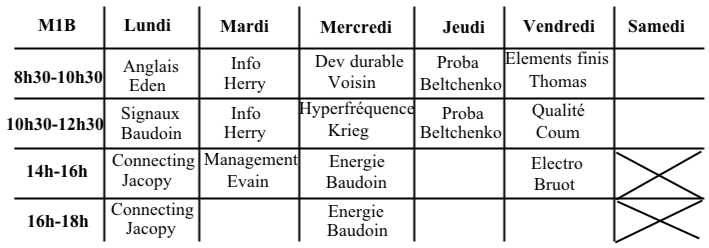
\includegraphics [width=110mm, height=45mm]{Dessin2.png}
\end{center}
\end{frame}

\subsection{Les professeurs}
\begin{frame} 
Les professeurs ont 4 paramètres : 
\begin{itemize}
\item l'identifiant
\item le nom
\item ses disponibilités
\item la liste des cours enseignés
\end{itemize}
\end{frame}

\begin{frame}
11 demi-journées par semaine\\

Prof disponible  $\rightarrow$ 1\\
Prof non disponible  $\rightarrow$ 0\\
\vspace{\baselineskip}
Représentation des disponibilités d'un professeur sur les semaines:
\begin{itemize}
\item 1111 0011 1100 0011 1111 00
\end{itemize}
\end{frame}

\subsection{Les classes}
\begin{frame}
Les classes ont 5 paramètres : 
\begin{itemize}
\item l'identifiant
\item le nom
\item la promotion à laquelle elle appartient
\item les cours à recevoir
\item le nombre d'élèves\\
\end{itemize}
\vspace{\baselineskip}
Promotions constituées de $n$ classes
\end{frame}

\subsection{Les matières}
\begin{frame}
Les matières ont 4 paramètres : 
\begin{itemize}
\item l'identifiant
\item le nom
\item la promotion
\item le nombre d'heures sur le semestre\\
\end{itemize}
\vspace{\baselineskip}
Matière en commun à 2 promotions : Algèbre B1, Algèbre B2\\ 
\end{frame}

\subsection{Les emplois du temps}
\begin {frame}
Un emploi du temps généré pour chaque classe : \\
\begin{itemize}
\item Contient l'ensemble des semaines du semestre
\item Chaque semaine contient les 22 créneaux
\item Un créneau contient : 
\begin {itemize}
\item le cours
\item le professeur
\end{itemize}
\end{itemize}
\end{frame}

\subsection{Les cours non placés}
\begin{frame}
Les cours qui n'ont pas pu être placés seront listés dans un fichier.
Chaque cours aura : 
\begin{itemize}
\item le cours
\item la promotion
\item le professeur
\item la semaine
\end{itemize}
\end{frame}



\section{Contraintes et conventions}

\subsection{Sur les professeurs}
\begin{frame}
\begin{itemize}
\item Un seul cours par créneau
\item Contraintes liées aux disponibilités
\item Un seul professeur par matière et par classe
\end{itemize}
\end{frame}

\subsection{Sur les semaines}
\begin{frame}
\begin{itemize}
\item Programme d'une semaine commun à chaque classe d'une même promotion
\item Cours de 4 heures sur une même demi-journée
\end{itemize}
\end{frame}

\subsection{Sur les classes}
\begin{frame}
\begin{itemize}
\item Un seul cours par créneau
\item Cours reportés sur le même créneau d'une semaine à l'autre
\item Un seul cours du même type par semaine
\item Pas de cours mélangeant plusieurs classes
\end{itemize}
\end{frame}



\section{Génération de l'emploi du temps}
\begin {frame}
Génération de l'emploi du temps à partir des données en entrée.

3 étapes de conception : 
\begin{itemize}
\item les pré-traitements
\item répartition du programme sur le semestre
\item emploi du temps spécifique à chaque classe
\end{itemize}
\end{frame}

\subsection{Pré-traitements}
\begin{frame}
Pré-traitement pour écarter les instances incohérentes\\
\vspace{\baselineskip}
Evaluation des critères suivants :
\begin {itemize}
\item nombre de professeurs
\item nombre d'heures de cours par promotion
\end{itemize}
\end{frame}

\begin{frame}
Pour chaque matière :
\begin{itemize}
\item Calcule le nombre d'heures que peuvent donner les professeurs.
\item Compare cette somme avec le nombre d'heures à dispenser
\end{itemize}
\vspace{\baselineskip}
Exemple :\\
Cours d'algèbre : 4 heures par semaine pour 6 promotions\\ 
$\rightarrow$ 24 heures à dispenser\\
Professeurs qualifiés : Dr Hagbe, 20 heures et M. Tort, 20 heures\\
$\rightarrow$ 40 heures de libre\\
\end{frame}

\begin{frame}
Evaluation du nombre d'heures :\\
\begin{itemize}
\item Calcule le temps nécessaire pour dispenser toutes les matières du programme
\item Compare cette somme avec le nombre total d'heures du semestre
\end{itemize}
\end{frame}


\subsection{Répartition du programme sur le semestre}
\begin{frame}
Objectifs :
\begin{itemize}
\item Déterminer un enchaînement logique des matières
\item Garantir l'homogénéité des cours au sein d'une promotion
\end{itemize}
\vspace{\baselineskip}
Méthode :
\begin{itemize}
\item Traiter les promotions indépendamment les unes des autres
\item Positionner les cours les plus volumineux au début du semestre
\end{itemize}
\end{frame}

\begin{frame}
Trie des cours
\begin{center}
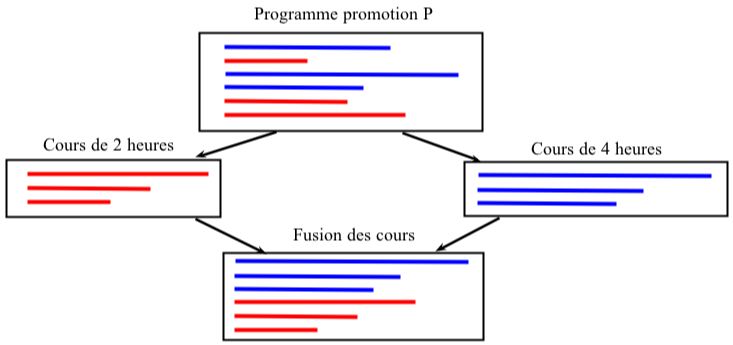
\includegraphics [width=117mm, height=60mm]{Dessin1.png}
\end{center}
\end{frame}

\begin{frame}
Mise en place des répartitions des cours sur le semestre
\begin{center}
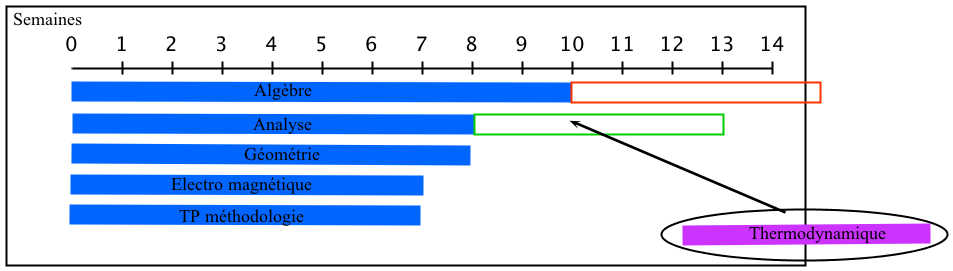
\includegraphics [width=117mm, height=60mm]{RepartitionSemestre2.png}
\end{center}
\end{frame}

\begin{frame}
Répartition du programme sur le semestre
\begin{center}
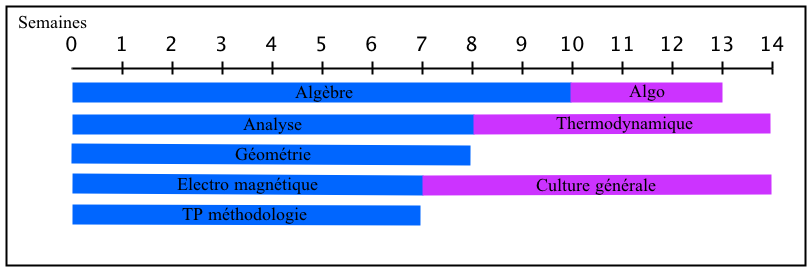
\includegraphics [width=110mm, height=60mm]{RepartitionSemestre.png}
\end{center}
\end{frame}

\subsection{Emploi du temps final}

\begin{frame}
Principe :
\begin{itemize}
\item Fonction de répartition aléatoire des cours dans la semaine.\\
\item Génération de $n$ emplois du temps jusqu'à trouver une solution satisfaisante\\ 
\item Création des emplois du temps par promotion
\end{itemize}
\end{frame}

\begin{frame}
Création d'un emploi du temps :\\
\begin{itemize}
\item Semaine par semaine
\item Pour toutes les classes de la promotion sélectionnée
\end{itemize}
\end{frame}

\begin{frame}
Emploi du temps d'une semaine :
\begin{itemize}
\item Identification du couple promotion-professeur ayant le moins de créneaux en commun
\item Choix aléatoire de l'un de ces créneaux
\item Placement effectif du cours dans l'emploi du temps de la classe
\item Mise à jour des disponibilités du professeur
\end{itemize}
\end{frame}

\begin{frame}
Enchaînement de semaines :
\begin{itemize}
\item Copie des cours non terminés la semaine précédente
\item Ajout des nouveaux cours de la même manière que précédemment
\end{itemize}
\end{frame}

\begin{frame}
\begin{center}
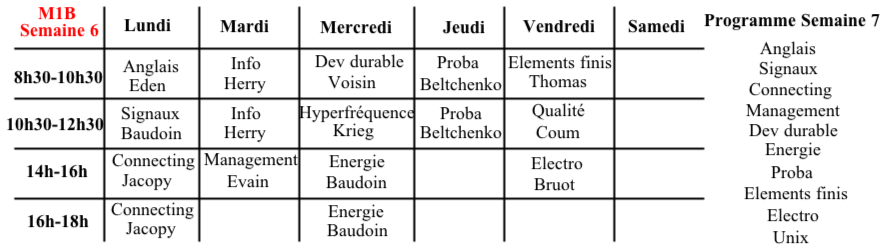
\includegraphics [width=110mm, height=45mm]{Dessin3.png}
\end{center}
\end{frame}

\begin{frame}
\begin{center}
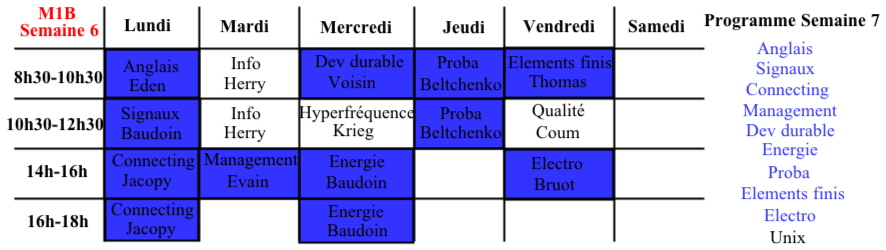
\includegraphics [width=110mm, height=45mm]{Dessin4.png}
\end{center}
\end{frame}

\begin{frame}
\begin{center}
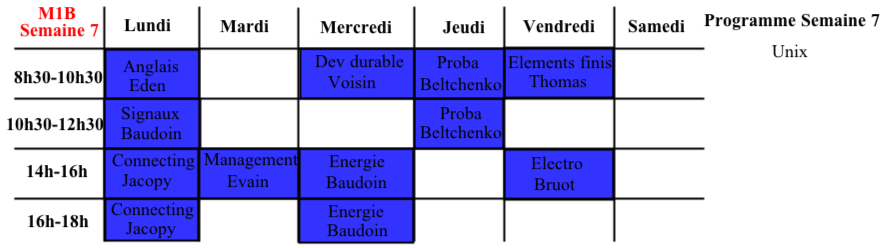
\includegraphics [width=110mm, height=45mm]{Dessin5.png}
\end{center}
\end{frame}

\begin{frame}
Exceptions :
\begin{itemize}
\item Cours de 4h non placé sur une demi-journée
\item Plus de créneau commun au professeur et à la promotion\\
\end{itemize}
Cours concernés ajoutés à la liste des cours non placés.
\end{frame}

\subsection{Déplacement de cours}
\begin{frame}
Deux types de déplacements :
\begin{itemize}
\item Placement d'un cours à partir de la liste des cours non placés
\item Déplacement d'un cours pour assurer la maintenance de l'emploi du temps
\end{itemize}
\end{frame}

\section{Bilan}
\subsection{Discussion}
\begin{frame}
Les améliorations possibles : 
\begin{itemize}
\item Les classes de M2
\item Les salles et les locaux
\item Les TP
\end{itemize}
\end{frame}

\subsection{Conclusion}
\begin{frame}
\begin{itemize}
\item Méthode heuristique trouvant une solution\\
\item Dans un temps correcte $\rightarrow$ 0,145 secondes\\
\item Interface homme-machine en cours de réalisation
\end{itemize}
\end{frame}

\end{document}